\documentclass[tikz,border=10pt]{standalone}
\usepackage{tikz}
\usetikzlibrary{positioning, fit, backgrounds}
\begin{document}
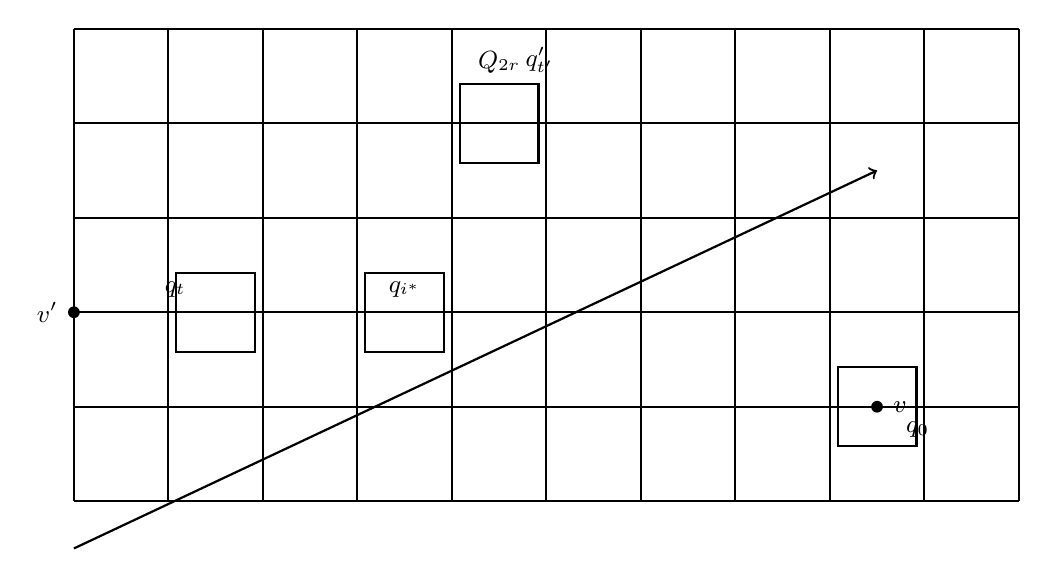
\begin{tikzpicture}[scale=1.2, font=\small]

% Define styles
\tikzset{
    cell/.style={minimum size=1cm, draw, thick},
    dot/.style={circle, fill, inner sep=1.5pt},
    line/.style={thick},
}

% Draw horizontal lines
\foreach \y in {0,...,5}{
    \draw[line] (-1,\y) -- (9,\y);
}

% Draw vertical lines
\foreach \x in {-1,...,9}{
    \draw[line] (\x,0) -- (\x,5);
}

% Draw the diagonal line
\draw[line,->] (-1,-0.5) -- (7.5,3.5);

% Draw specific rectangles and nodes
\node[cell, label={north:$Q_{2r}$}] (q2r) at (3.5,4) {};
\node[cell] (qt) at (0.5,2) {};
\node[cell] (qi*) at (2.5,2) {};
\node[cell] (q0) at (7.5,1) {};

% Place dots
\node[dot, label={west:$v'$}] (vprime) at (-1,2) {};
\node[dot, label={east:$v$}] (v) at (7.5,1) {};

% Add labels
\node[anchor=north] at (qt.north west) {$q_t$};
\node[anchor=north] at (qi*.north) {$q_{i^*}$};
\node[anchor=south] at (q0.south east) {$q_0$};
\node[anchor=south] at (q2r.north east) {$q'_{t'}$};

\end{tikzpicture}
\end{document}